\scanpage{69}
\margin{68}
\mspage{10}
dans la carte triangulée pondérée envisagée, les sommets de type $i$ \deleted{sont d'}\inserted{ont un} ordre réduit \uline{divisant} $\nu_i$. Une telle condition peut être introduite pour un ou plusieurs indices $i$. Dans le cas des cartes ordinaires (interprétées comme définissant une triangulation pondérée, via la subdivision barycentrique) une relation
\[
\text{(30)}\qquad \rho_0^{\nu_0}=1\qquad(\text{resp. }\rho_\infty^{\nu_\infty}=1)
\]
signifie que les sommets sont d'ordre divisant $\nu_0$ (resp. que les faces sont d'ordre divisant $\nu_\infty$).

Quant à la relation
\[
\text{\deleted{\unsure{(31)}}\unsure{(*)}}\qquad \rho_1^{\nu_1}=1,
\]
comme on a déjà $\rho_1^2=1$, ou bien $\nu_1$ est \inserted{pair} et cette relation$^{\unsure{(*)}}$ est automatiquement satisfaite, ou bien $\nu_1$ est impair, et elle implique
\[
\rho_1=1
\]
ce qui signifie que la carte correspond à un revêtement de $\mathbb P^1_{\mathbb C}$ ramifié seulement en $0$ et $\infty$, donc à un revêtement ``cyclotomique'' $z\mapsto z^n$ ($n\in\mathbb N$), \deleted{cas qui} donnant lieu à \deleted{des} cartes régulières \inserted{sphériques} de groupe $\mathbb Z/n\mathbb Z\simeq\mu_n(\mathbb C)$ ayant un seul sommet, une seule face, et $n$ arêtes disposées circulairement (carte isomorphe à sa duale, visiblement) -- ce qui est relativement trivial. Donc on peut dire
\figure{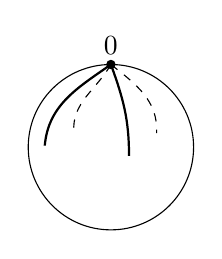
\begin{tikzpicture}
\draw (0,0) circle (1.05);
\fill (0,1.05) circle (.06); \node[above] at (0,1.05) {$0$};
\draw[thick] (0,1.05) to[out=-145,in=85] (-.84,.02);
\draw[thick] (0,1.05) to[out=-70,in=90] (.23,-.11);
\draw[dashed] (0,1.05) to[out=-120,in=95] (-.47,.18);
\draw[dashed] (0,1.05) to[out=-38,in=87] (.58,.18);
\end{tikzpicture}}
